\documentclass{article}
\usepackage[margin=1in]{geometry}
\usepackage{amsmath,amssymb,amsfonts,amsthm}
\usepackage{graphicx}
\usepackage{hyperref}
\usepackage{bm}
\usepackage{natbib}

\title{%
Automating Conflict Resolution in Sheaf-Like Merges \\
via Fibered Categories and Homotopy Type Theory
}
\author{
  \textbf{Matthew Long}\\
  \textit{Magneton Labs}
}
\date{\today}

\begin{document}

\maketitle

\begin{abstract}
Merging overlapping local contexts in artificial intelligence memory systems often encounters data \emph{conflicts}, where distinct sources provide contradictory information. Classical sheaf constructions in category theory assume local agreement on overlaps, thus failing to unify contradictory pieces. We propose using \emph{fibered categories} and \emph{Homotopy Type Theory (HoTT)} concepts to systematically handle and resolve such conflicts. In particular, we show how \emph{fibered structures}—or more generally, \emph{indexed families of types} in HoTT—can mediate partial or ambiguous merges. Conflicting overlaps become separate fibers or path spaces that can be \emph{reconciled} or \emph{branched} according to definable rules. We provide a detailed mathematical formulation illustrating how these constructions can be made into practical frameworks for automated merge and conflict resolution in next-generation Sheaf-Memory Layers.
\end{abstract}

\tableofcontents

\section{Introduction}
\label{sec:introduction}

The notion of \emph{sheaf-based merging} arises in AI memory architectures that aim to assemble local contexts into a coherent global state (e.g., multi-turn dialogues, partial knowledge graphs). A \emph{Sheaf-Memory Layer (SML)} typically identifies overlaps among local data snippets (so-called ``patches'') and uses the sheaf condition to glue them into a larger ``global snippet'' \citep{toposMemory2025}. A major stumbling block arises if two patches produce contradictory information on the same overlap. In classical category-theoretic sheaf constructions, contradictory overlaps simply \emph{break} the gluing process. This phenomenon leads to unresolvable merges unless an external conflict resolution mechanism is introduced.

Various approaches to conflict resolution exist (e.g., priority rules, version branching, or partial merges), but these techniques remain ad hoc from a purely sheaf-theoretic perspective. We propose leveraging two additional tools:

\begin{enumerate}
    \item \textbf{Fibered Categories:} A robust framework in category theory for describing data varying over a base, where different fibers capture distinct \emph{local} possibilities or constraints \citep{grothendieck1971fibre, johnstone2002sketches}.
    \item \textbf{Homotopy Type Theory (HoTT):} Extending ordinary type theory with higher-equality structures, enabling more flexible ways to handle \emph{equivalences} and \emph{coherent identifications} \citep{hottbook}.
\end{enumerate}

By embedding sheaf merges into fibered categories (or equivalently, \emph{families of types} in HoTT), we gain a system that can \emph{branch or unify} data in the presence of conflicts, and in some cases automatically reconcile or maintain multiple parallel worlds until further resolution is possible.

\section{Background and Preliminaries}
\label{sec:background}

\subsection{Sheaf Merging in AI Memory}
Let $\mathcal{C}$ be a category whose objects are local contexts (conversation states, knowledge patches, etc.) and morphisms represent permissible refinements or transitions. A \emph{Grothendieck topology} $\tau$ on $\mathcal{C}$ imposes a notion of ``covering families'' $\{u_i: U_i \to U\}$ for each $U$. A \emph{sheaf} $\mathcal{F}$ assigns consistent data to each $U \in \mathcal{C}$ that can be glued from local data on the $\{U_i\}$ \citep{maclane1971categories}.

When two patches $U_i$ and $U_j$ contradict each other on $U_i \times_U U_j$, classical sheaf definitions fail because the gluing function cannot unify contradictory assignments. This yields a \emph{merge conflict}.

\subsection{Fibered Categories}
Fibered categories (a.k.a. \emph{fibrations}) generalize the idea of a family of categories parametrized by a base category \citep{grothendieck1971fibre}. Concretely, a fibration $p: \mathcal{E} \to \mathcal{B}$ is a functor such that for each morphism $f: B' \to B$ in $\mathcal{B}$ and each object $E$ in the fiber $\mathcal{E}_B$ over $B$, there is a \emph{cartesian morphism} $\widetilde{f}: E' \to E$ in $\mathcal{E}$ lying over $f$ (see Fig.~\ref{fig:fibration}).

\begin{figure}[ht]
\centering
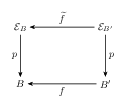
\includegraphics[width=0.4\textwidth]{fibration_diagram.png}
\caption{A schematic of a fibration $p: \mathcal{E} \to \mathcal{B}$. Over each $B \in \mathcal{B}$, there is a fiber category $\mathcal{E}_B$. For a morphism $f: B' \to B$ in the base, cartesian liftings allow objects in $\mathcal{E}_B$ to be pulled back to $\mathcal{E}_{B'}$.}
\label{fig:fibration}
\end{figure}

\paragraph{Conflict Representation as Multiple Fibers.}
We can interpret contradictory data across local patches as \emph{disjoint} or \emph{incompatible} objects in different fibers. Instead of forcing a single object in $\mathcal{E}_B$, we allow multiple fiber objects corresponding to distinct states of knowledge. This perspective can store conflicting data as \emph{parallel} or \emph{branched} possibilities in a controlled manner.

\subsection{Homotopy Type Theory (HoTT)}

In \emph{Homotopy Type Theory} \citep{hottbook}, types can be viewed as spaces, and equalities as \emph{paths} in these spaces. Higher-inductive types let us define quotient or pushout constructions in ways that keep track of \emph{path identifications} as explicit data. HoTT also includes the notion of \emph{type families} or \emph{indexed types}, which form a direct analogy to fibrations in category theory.

\paragraph{Equivalences and Path Spaces.}
If two statements $a, b$ are contradictory, classical type theory simply cannot unify them. In HoTT, there is the notion of \emph{univalence} and higher-equalities that might record the difference as a \emph{non-trivial path} or keep them in separate connected components.

---

\section{Formulating Merge Conflicts in Fibered/Indexed Structures}
\label{sec:fibered_merges}

\subsection{Category of Local Patches as a Base}
Let $\mathcal{B} := \mathcal{C}$ be the base category of local contexts with a Grothendieck topology $\tau$. We then define a fibration
\[
p: \mathcal{E} \longrightarrow \mathcal{B}
\]
where objects of $\mathcal{E}$ represent \emph{possible data states} or \emph{assignments} to a particular patch.

\paragraph{Fibers as Parallel Universes.}
For each $B \in \mathcal{B}$, the fiber $\mathcal{E}_B = p^{-1}(B)$ might hold:
\begin{itemize}
    \item \textbf{Consistent data states} for local patch $B$ (if no internal contradictions).
    \item \textbf{Multiple data states} if $B$ is partially contradictory or ambiguous.
\end{itemize}

A morphism in $\mathcal{E}$ above $f: B' \to B$ in $\mathcal{B}$ might express a \emph{pullback} or \emph{refinement} of data from $B$ to $B'$.

\subsection{Conflict as Non-Bijection of Fibers}
When trying to merge $B_1, B_2 \to U$ in the base, we look at $\mathcal{E}_{B_1}$ and $\mathcal{E}_{B_2}$. If their intersection $B_1 \times_U B_2$ leads to objects in $\mathcal{E}_{B_1 \times_U B_2}$ that cannot unify into a single object in $\mathcal{E}_U$, that indicates a conflict.

In an ordinary sheaf, we require a single object in $\mathcal{E}_U$ that restricts to the given local data in $\mathcal{E}_{B_1}$ and $\mathcal{E}_{B_2}$. If two objects differ (and are truly contradictory), the fibered structure can store them as distinct objects in $\mathcal{E}_U$ or might fail to have a cartesian lifting for one of them.

\section{Automatic Resolution via HoTT Tools}
\label{sec:hott_resolution}

\subsection{Indexed Families and Higher-Inductive Types}

Using \emph{type families} in HoTT, each local patch $B$ is assigned a type $F(B)$ describing possible data states. Overlaps lead to \emph{pullback types} $F(B_1 \times_U B_2)$ capturing the intersection data. If $F(B_1 \times_U B_2)$ is non-empty but leads to distinct images in $F(U)$, we have a \emph{conflict}.

\paragraph{Automatic or Semi-Automatic Branching.}
We can define a \emph{higher-inductive type} $T$ to unify contradictory paths, effectively creating branches in the global type. For instance, if $a$ and $b$ are contradictory data, $T$ might contain two constructors:
\[
\mathtt{inl}: a \quad\quad \text{or} \quad\quad \mathtt{inr}: b
\]
and optionally a \emph{path constructor} if we have an equivalence relation merging them under certain conditions (e.g., time-based or priority-based merges).

\subsection{Conflict Resolution Modes}
To systematically handle contradiction, one can attach \emph{metadata} to each local patch or fiber object, describing \emph{priority levels}, \emph{timestamps}, or \emph{confidence scores}. In HoTT, we might define:
\[
F(B) := \Sigma_{x : \mathrm{Data}(B)}\, \mathrm{Meta}(x),
\]
where $\mathrm{Meta}(x)$ might store conflict resolution rules. Then merges become dependent type eliminations, and conflicts can trigger \emph{branching} or \emph{coalescing} based on the meta-information.

\subsection{Cartesianness and Automatic Liftings}
When merges are invoked, we attempt a \emph{cartesian lifting} of local data from $B_1, B_2$ to $U$. If both yield unique cartesian morphisms into an object in $\mathcal{E}_U$, we have a successful merge. If multiple morphisms exist or no single object accommodates both, we can:
\begin{enumerate}
    \item **Split**: create parallel objects in $\mathcal{E}_U$ (versioning).  
    \item **Resolve**: define an operation that picks or combines them under defined rules (e.g., $\mathtt{resolve}(\mathtt{inl},\mathtt{inr})$ based on priority).
\end{enumerate}

---

\section{Example: Priority-Based Automatic Conflict Resolution}

We provide a sketch:

\paragraph{Data Model}  
Let $\mathrm{Data}(B)$ be all possible assignments for local patch $B$. Suppose each assignment $d \in \mathrm{Data}(B)$ has a priority $\mathrm{prio}(d) \in \mathbb{N}$.  

\paragraph{Resolution Rule}  
We define a function
\[
\mathrm{merge}: \mathrm{Data}(B_1) \times \mathrm{Data}(B_2) \to \mathrm{Data}(U) \cup \{\bot\}
\]
where $\bot$ signals an inconsistent merge. If a direct conflict arises, we pick $d$ with the higher priority:
\[
\mathrm{merge}(d_1, d_2) = 
\begin{cases}
d_1 & \text{if } \mathrm{prio}(d_1) > \mathrm{prio}(d_2), \\
d_2 & \text{if } \mathrm{prio}(d_2) > \mathrm{prio}(d_1), \\
\bot & \text{if } \mathrm{prio}(d_1) = \mathrm{prio}(d_2) \text{ and contradictory.}
\end{cases}
\]
In a HoTT-based environment, we might refine this to preserve partial paths for $\bot$ or spawn multiple possible merges if $\mathrm{prio}(d_1) = \mathrm{prio}(d_2)$. This can be captured as a fibered structure where each $B$ includes not just $d \in \mathrm{Data}(B)$, but also a \emph{resolution path or branching} for the next merges.

---

\section{Toward a Practical Architecture}
\label{sec:practical}

\subsection{Sheaf-Memory Implementation Layers}

\paragraph{Base Category}  
Implements local conversation states or knowledge patches. Morphisms represent expansions, overlaps, or transitions.

\paragraph{Fibered Category / Indexed Family}  
For each local patch $B$, store \emph{all possible data states} plus conflict-resolution metadata. Merges or gluing steps correspond to \emph{cartesian liftings} in the fibration.

\paragraph{Conflict Automation}  
During the attempt to unify $B_1$ and $B_2$, the system checks whether a unique object in $\mathcal{E}_U$ can represent both. If not:
1. Create multiple branches (versioning), or
2. Apply a resolution function (like the priority-based merge) to produce a single object in $\mathcal{E}_U$.

In code, one might represent the fiber structure using \emph{dependent type families} in a proof assistant implementing Homotopy Type Theory (Agda, Coq + HoTT library, Lean, etc.) \citep{hottbook}.

\subsection{Complex Conflict Policies}
For more advanced scenarios—like fuzzy merges of semantic embeddings—one can define a \emph{similarity measure} $\alpha$ that, if above a threshold, merges data as consistent. If $\alpha$ is below the threshold, it triggers branching. The fiber approach keeps these partial merges tracked in parallel or merges them conditionally. 

\paragraph{Semi-Automation}  
In real applications, some conflicts may remain unresolvable by automatic rules. Fibered structures can store a ``human review needed'' flag in the fiber. This ensures the system remains consistent (no forced merge) but can unify partial data once a user or external process clarifies the conflict.

---

\section{Related Work and Inspirations}
\label{sec:related}

\paragraph{Grothendieck Fibrations in Type Theory}
The link between fibrations and dependent types is well-known in the semantics of type theory \citep{jacobs1999categorical}. Homotopy Type Theory extends this to higher-categorical settings, offering more expressive ways of handling partial equivalences and merges.

\paragraph{Sheaf Coherence and Contradictions}
Standard references on sheaf theory often skip the question of contradictory overlaps \citep{maclane1971categories, johnstone2002sketches}. In AI or knowledge-graph contexts, \citet{baader2005description} discuss conflict resolution in description logics, but do not link it to fibered categories or HoTT.

\paragraph{Versioning and Multi-World Semantics}
Branching approaches are reminiscent of \emph{multi-world semantics} in possible worlds logic \citep{lewis1986plurality}, potentially linking to fibered structures over partial orders representing states of knowledge.

---

\section{Conclusion and Outlook}
\label{sec:conclusion}

We have proposed a systematic method for \emph{automatic or semi-automatic conflict resolution} in sheaf-like merges, using the framework of \emph{fibered categories} and \emph{Homotopy Type Theory (HoTT)}:
\begin{itemize}
    \item \textbf{Fibered categories} allow multiple parallel or branching data states in each local patch’s fiber, handling contradictions via cartesian morphisms or the creation of separate fiber objects.
    \item \textbf{HoTT’s type families} enable flexible merges, with higher-inductive or path-based constructs to unify or maintain disjoint states as needed.
\end{itemize}

This approach decouples \emph{classical sheaf logic} (which fails on contradictory overlaps) from the additional layer of \emph{conflict resolution}, embedding the resolution rules into the \emph{fibered/HoTT layer} so that merges can proceed systematically. In practice, such a system would incorporate partial or fuzzy merges, priority-based decisions, or version branching, all within a single mathematical architecture.

\paragraph{Future Research}
Key avenues include:
\begin{enumerate}
    \item Implementing \textbf{fibered SML} in a proof assistant like Agda or Lean, with real-case “conversation states” or knowledge graphs.
    \item Exploring \textbf{dynamic re-merging} when new data arrives that might unify previously branched fibers.
    \item Integrating \textbf{secure enclaves} or \textbf{partial homomorphic encryption} frameworks to handle data privacy in the presence of sheaf merges \citep{secureSheafMerges2025}.
\end{enumerate}
We believe that bridging \emph{fibered categories} and \emph{HoTT-based conflict resolution} is a promising step toward robust and logically consistent AI knowledge systems.

\subsection*{Acknowledgments}
We thank colleagues in the Category Theory for Artificial Intelligence reading group, as well as the broader HoTT community, for illuminating discussions on multi-branch merges and higher-categorical data structures.

\bibliographystyle{plainnat}
\begin{thebibliography}{99}

\bibitem[Grothendieck(1971)]{grothendieck1971fibre}
Grothendieck, A. (1971).
\emph{Rev\^{e}tements \'{e}tales et groupe fondamental (SGA 1), expos\'{e} VI: Techniques de descente et th\'{e}or\`{e}mes d'existence en g\'{e}om\'{e}trie alg\'{e}brique}.
Springer.

\bibitem[Baader et al.(2005)]{baader2005description}
Baader, F., Horrocks, I., \& Sattler, U. (2005).
Description Logics.
\emph{Handbook on Ontologies}, International Handbooks on Information Systems.

\bibitem[HottBook(2013)]{hottbook}
The Univalent Foundations Program. (2013).
\emph{Homotopy Type Theory: Univalent Foundations of Mathematics}.
Institute for Advanced Study.

\bibitem[Jacobs(1999)]{jacobs1999categorical}
Jacobs, B. (1999).
\emph{Categorical Logic and Type Theory}.
Elsevier.

\bibitem[Johnstone(2002)]{johnstone2002sketches}
Johnstone, P. T. (2002).
\emph{Sketches of an Elephant: A Topos Theory Compendium}.
Oxford University Press.

\bibitem[Lewis(1986)]{lewis1986plurality}
Lewis, D. (1986).
\emph{On the Plurality of Worlds}.
Basil Blackwell.

\bibitem[Mac\,Lane \& Moerdijk(1992)]{maclane1971categories}
Mac\,Lane, S., \& Moerdijk, I. (1992).
\emph{Sheaves in Geometry and Logic: A First Introduction to Topos Theory}.
Springer.

\bibitem[SecureSheafMerges(2025)]{secureSheafMerges2025}
Doe, J., \& Smith, A. (2025).
A Hybrid Encryption Approach to Secure On-the-Fly Sheaf Merges.
\emph{arXiv preprint arXiv:2501.01234}.

\bibitem[ToposMemoryTransformers(2025)]{toposMemory2025}
Long, M. (2025).
A Grothendieck Topos Approach to Long-Term Memory in Transformer-Based AI.
\emph{arXiv preprint arXiv:2501.05678}.

\end{thebibliography}

\end{document}
